\documentclass[a4paper,11pt]{article}
\usepackage[left=0.85in,right=0.85in,top=0.80in,bottom=0.80in]{geometry}
\usepackage{listings}
\usepackage{amsmath}
\usepackage{fmtcount}
\usepackage{datetime}
\usepackage[pdftex]{graphicx}
\usepackage{caption}
\usepackage{subcaption}
\usepackage{fancyhdr}
\usepackage{color}
\usepackage{fancyvrb}

\usepackage{tabu}
\usepackage{xcolor}\newcommand{\squeezeup}{\vspace{-7mm}}
\begin{document}
\begin{center}
{\Huge Problem ID: kerning}\vspace{2 mm} \\	% Problem Letter
{\huge Kerning}\vspace{2 mm} \\	% Problem Name
\end{center}
\setcounter{page}{9}
\large{
In typography, \emph{kerning} is the process of adjusting the spacing between characters (also known as \emph{glyphs}) in a font. A well-kerned font is one where the spacing between individual characters is visually appealing. Fonts are typically represented as a two dimensional array of bit pixels (black or white) where glyphs are placed side by side and are kerned appropriately.\\
\begin{figure}[!htb]
    \centering
    \begin{minipage}{.5\textwidth}
        \centering
        
\includegraphics[width=0.5\linewidth, height=0.05\textheight]{hw.jpg}
        \caption{A well(ish)-kerned font represented as a bitmap.}
    \end{minipage}%
    \begin{minipage}{0.5\textwidth}
        \centering
        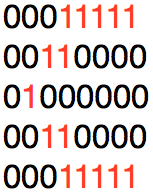
\includegraphics[width=0.32\linewidth, height=0.143\textheight]{bitmap.png}
        \caption{A 5x8 bitmap. The glyph is highlighted in red.}
    \end{minipage}
\end{figure}
\\
Let's say that `1' represents a bit pixel that is part of a glyph and `0' represents a bit pixel that is part of the background. Then, we formally define a glyph as a maximal set of `1' bit pixels with the property that we can find a path from every bit pixel in the set to every other one (a path consisting of only up/down, left/right, and diagonal moves). Suppose we are given a bitmap that contains exactly two glyphs. The \emph{level of kerning} between these two glyphs is the minimum distance between any point of the first and second glyph (where distance is measured using the square of the euclidean distance). More specifically, the distance between two points $(x_0, y_0)$ and $(x_1, y_1)$ is $(x_0-x_1)^2 + (y_0-y_1)^2$; the first coordinate is the row number (starting at the top as 0) and the second coordinate is the column number (starting from the left as 0).
}
\vspace{7mm}\\
\large{\bf{Input}}\vspace{2mm}\\
The input will begin with a line containing a single positive integer, $t$, representing the number of test cases to process. Each test case will begin with a single line containing two space-separated integers $N$ and $M$ ($1 \leq N, M \leq 100$) each representing number of rows and columns in the bitmap, respectively. Following will be $N$ lines each containing $M$ characters (which will be either '0' or '1') which collectively are the bitmap for this test case. It is guaranteed that each bitmap will contain \emph{exactly} two glyphs.
\vspace{3mm}\\
\large{\bf{Output}}\vspace{2mm}\\
For each test case print the level of kerning between the two glyphs on its own line.
\vspace{110mm}\\
\bf{Sample Input} \hspace{52mm} \bf{Sample Output}\vspace{1mm}\\
\begin{tabu*} to 475pt {|X[0r]|X[0l]|}
\tabucline-
\vspace{-\baselineskip} %needs to be placed here
\begin{Verbatim}
2
6 20 
00000000000000000000
11111111000011000000
00011000000011000000
00011000000011100000
00011000000011111110
00000000000000000000
5 10
0000111000
0010001000
1110001000
0010001000
0000000100
\end{Verbatim}
&
\vspace{-\baselineskip} %needs to be placed here
\begin{Verbatim}
25
5
\end{Verbatim}
\\
\tabucline-
\end{tabu*}
\end{document}
